% !TEX TS-program = XeLaTeX

\documentclass[12pt, notitlepage]{ctexbook}
\usepackage{xeCJK}
\usepackage[font=small]{caption}
\usepackage{tikz}
\usepackage{fancyhdr}
\usepackage{amsmath}
\usepackage{graphicx}
\usepackage{xcoffins}
\usepackage{xcolor}
\usepackage{fontspec}
\usepackage[a4paper]{geometry}
\usepackage{setspace}
\usepackage{emptypage}
\usepackage{titlesec}
\usepackage[breaklinks,colorlinks,linkcolor=black,citecolor=black,urlcolor=black]{hyperref}
% Set up commands for title page generation
\definecolor{ethblue}{RGB}{31, 64, 122}


\newfontfamily\dinprobold{KaiTi}
\newfontfamily\dinproregular{FandolHei}
\newfontfamily\dinprolight{KaiTi}
\graphicspath{ {images/} }
\newcommand\chapterdecoration{%
	\begin{tikzpicture}[remember picture,overlay,shorten >= -10pt]
	\filldraw[black,line width=0,rounded corners=0] (0,2.5) rectangle (\linewidth,2.55);
	\end{tikzpicture}%
}
\titleformat{\chapter}[display]%
{\heiti\zihao{1}}%
{第\zhnumber\thechapter 章}{10pt}%
{}[\vspace*{2cm}\chapterdecoration]

\begin{document}

	\pagestyle{plain}
	\NewCoffin \result
\NewCoffin \anchor
\NewCoffin \topbox
\NewCoffin \ethlogo
\NewCoffin \imagebox
\NewCoffin \textbox
\NewCoffin \departmentlogo
\NewCoffin \textboxtext
\NewCoffin \textboxsubtext
\NewCoffin \authortext

\SetHorizontalCoffin \result {}
\SetHorizontalCoffin \topbox {\color{ethblue}\rule{220mm}{3cm}}
\SetHorizontalCoffin \imagebox {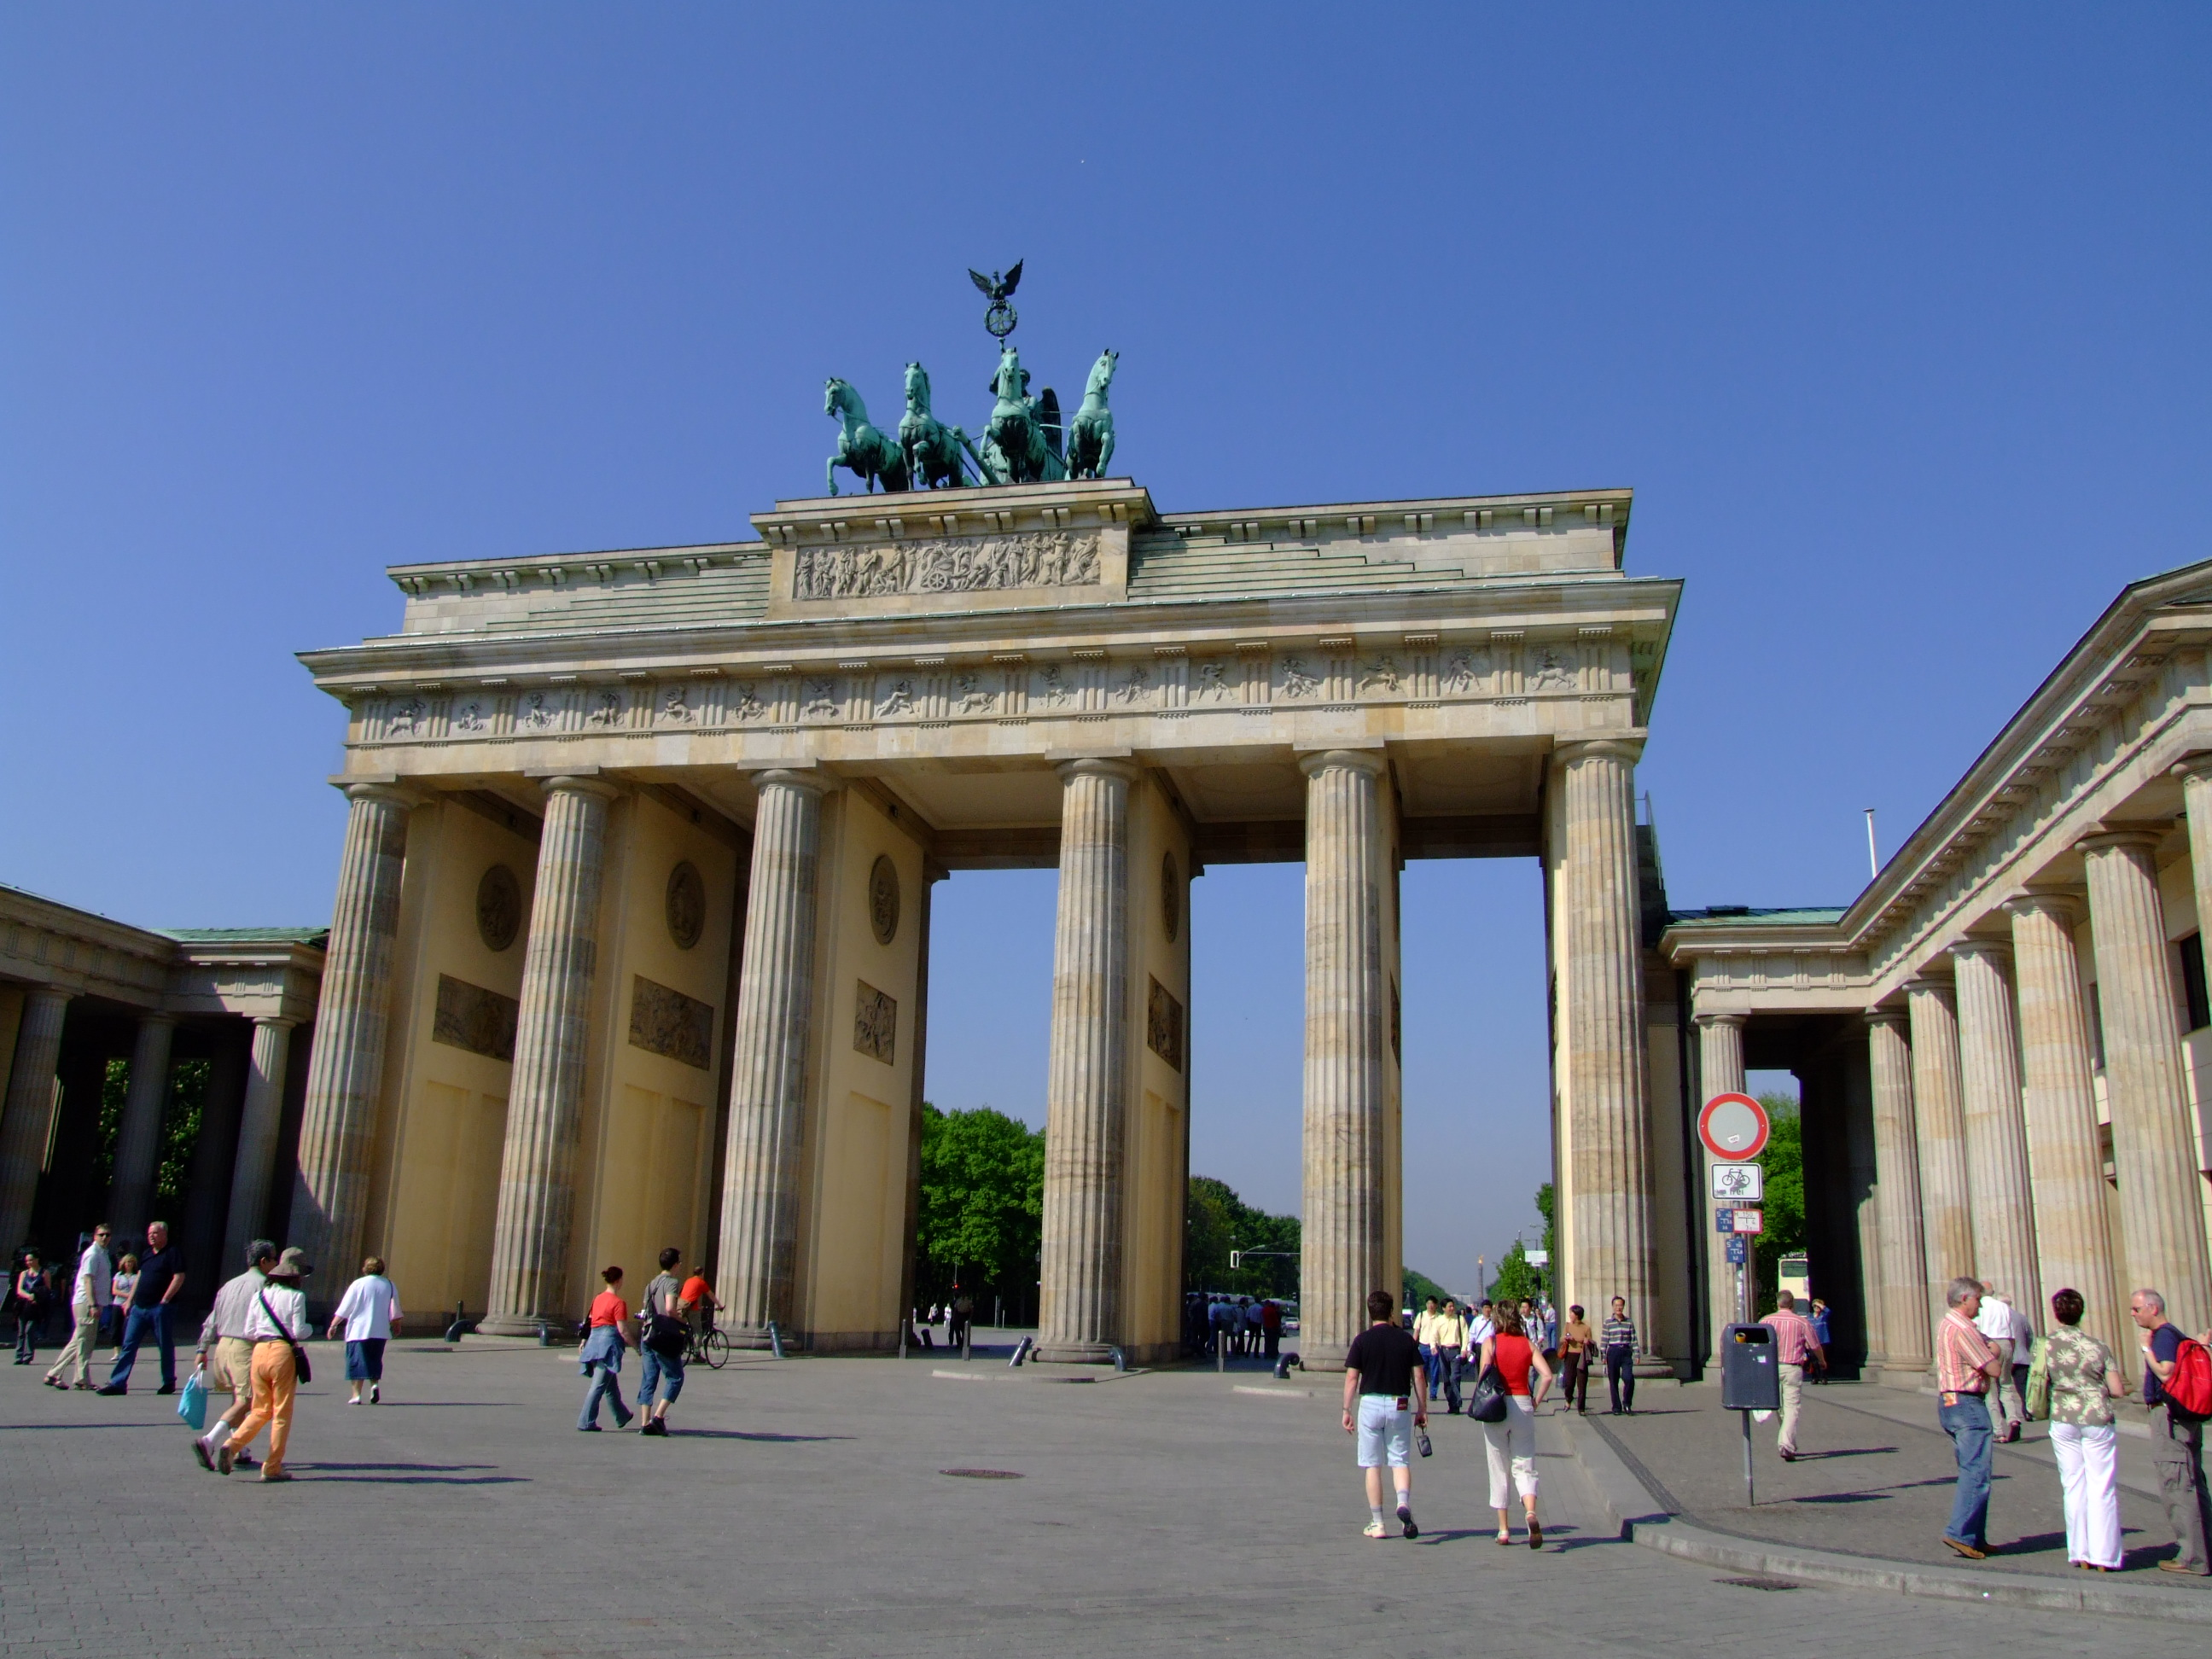
\includegraphics[width=190mm]{haupt}}
%\SetHorizontalCoffin \ethlogo {\includegraphics[width=50mm]{ethlogo}}
\SetHorizontalCoffin \textbox {\color{ethblue}\rule{190mm}{100mm}}
\SetVerticalCoffin \textboxtext {160mm} {\fontsize{40}{48}\dinprobold\noindent\textcolor{white}{CDAI文化指南}}
\SetVerticalCoffin \textboxsubtext {160mm} {\fontsize{21}{25}\dinproregular\noindent\textcolor{white}{中德文化差异小百科}}
\SetVerticalCoffin \authortext {160mm} {\flushright\fontsize{10}{12}\dinprolight\noindent\textcolor{white}{\today}}
\SetHorizontalCoffin \departmentlogo {
\includegraphics[width=30mm]{logo}}

% Positioning Hax
\JoinCoffins \result \topbox
\JoinCoffins \result[\topbox-hc, \topbox-b] \imagebox [hc, t](0mm,10mm)
\JoinCoffins \result[\imagebox-l, \imagebox-t] \ethlogo [l, b](0mm,5mm)
\JoinCoffins \result[\imagebox-l, \imagebox-b] \textbox [l, t](0mm,0mm)
\JoinCoffins \result[\textbox-hc, \textbox-t] \textboxtext [hc, t](-5mm, -5mm)
\JoinCoffins \result[\textboxtext-l, \textboxtext-b] \textboxsubtext [l, t](0mm, -5mm)
\JoinCoffins \result[\textbox-r, \textbox-b] \authortext [r, b](-5mm, 5mm)
\JoinCoffins \result[\textbox-l, \textbox-b] \departmentlogo [l, t](-5mm, -5mm)


% Generate the page
\thispagestyle{empty}
\newgeometry{left=0mm,bottom=0mm, top=0mm, right=0mm}
\noindent\TypesetCoffin \result
\restoregeometry
	\cleardoublepage
	\thispagestyle{empty}
	\begin{titlepage}
	\centering
	\vspace*{6cm}
	\noindent
	\center
	\begin{minipage}{0.7\linewidth}
	\zihao{0}\heiti CDAI文化指南\par
	\vspace{12pt}
	\zihao{-2}\songti ——中德文化差异百科\par
	\vspace{8cm}
	\heiti\zihao{-3}
	%
\includegraphics{logo}
	\raggedright
	项目成员:\\
	
	\vspace*{1em}
	\zihao{4}
	黄伟根\\
	黄耀鑫 \hspace{1em} 杨星林 \hspace{1em} 詹均升 \\
	张嘉伟 \hspace{1em} 周功豪 \hspace{1em} 周鹏 \\
	\end{minipage}
	\end{titlepage}

	\cleardoublepage
	\pagenumbering{roman}
	 \vspace*{3cm}
\begin{minipage}{\linewidth}
    \Huge\heiti\center{封面图片} \par
\end{minipage}

 \vspace*{3cm}

\par
勃兰登堡门位于德国首都柏林的市中心,最初是柏林城墙的一道城门,因通往勃莱登堡而得名。现在保存的勃莱登堡门是一座古典复兴建筑,由普鲁士国王腓特烈·威廉二世下令于1788年至1791年间建造,以纪念普鲁士在七年战争取得的胜利。
\cleardoublepage

\begin{minipage}{\linewidth}
\Huge\heiti\center{关于本书} \par
\end{minipage}

 \vspace*{3cm}
 %\normalfont\normalsize
 %\raggedright
 %\indent
 中国和德国都是世界上具有重大影响力的国家,随着传播 通讯技术的改进,交通技术的进步和经济的高度全球化,两国的合作越来越频繁。 然而,由于文化背景的不同,两国人民在交往的过程中不能够相互理解,,导致交际不能顺利进行。针对中德工程师学院和德国的应用技术大学之间日益频繁的交流活动,作为中德工程师学院的学生我们希望将一些所闻所知的一些信息整理、归类,尽可能为两国的学生做一些提示。本书不求包罗万象,但求准确,详尽,有趣。

\par
 在上学期,我们小组成员在项目发起人Frau Schneider的引领和指导下,为了增进我院及合作院校中、德两国学生间的文化认同感,减轻乃至消除文化差异所带来的沟通障碍,同时也为了我院新生能够更快适应和融入国际化的教学方式,多元化的人文环境,开展了一系列关于中德文化差异的研讨会、采访、问卷调查和现场调研。我们最终决定将项目的视角聚焦在七个文化主题上:服饰、饮食、体育、工作、交通、文化、卫生,以Wiki为载体,以百科全书式的写作手法,从学生的视角出发,独特地展现出我们对于异国文化的认识与思考。在项目期间,我们充分运用所学项目管理的知识,通过Projekt Auftrag, Zeitplan, PSP等项目管理工具控制项目进程;通过查阅相关资料、与德国师生互相交流讨论,并根据实际的生活体验,确定了各项主题的具体内容,并定期向同学与老师展示工作成果。项目的最后,我们的成果是喜人的,我们的中德文化差异百科全书在学院官网上线,向中德师生展现了中德文化大花园的一隅,虽然项目仍有不少改进的空间,但是我们希望通过这个学期的共同努力,把中德文化差异百科这座文化桥梁打造的更加坚固、优美。 相比于上学期, 这学期我们将从中德两国人民的日常行为差异入手,深入分析每个差异代表的文化内涵。我们希望通过这些方法,使中德两国国学生增进理解,弥合文化差异的鸿沟。
 \par
 在中国有一个小故事,讲的是汉朝的时候,在西南方有个名叫夜郎的小国家,它虽然是一个独立的国家,可是国土很小,百姓也少,物产更是少得可怜。但是由于邻近地区以夜郎这个国家最大,从没离开过国家的夜郎国国王就以为自己统治的国家是全天下最大的国家。有一天,夜郎国国王与部下巡视国境的时候,他指着前方问说:“这里哪个国家最大呀?”部下们为了迎合国王的心意,于是就说:“当然是夜郎国最大啰!”走着走着,国王又抬起头来、望着前方的高山问说:“天底下还有比这座山更高的山吗?”部下们回答说:“天底下没有比这座山更高的山了。”后来,他们来到河边,国王又问:“我认为这可是世界上最长的河川了。”部下们仍然异口同声回答说:“大王说得一点都没错。”从此以后,无知的国王就更相信夜郎是天底下最大的国家。有一次,汉朝派使者来到夜郎,途中先经过夜郎的邻国滇国,滇王问使者:“汉朝和我的国家比起来哪个大?”使者一听吓了一跳,他没想到这个小国家,竟然无知的自以为能与汉朝相比。却没想到后来使者到了夜郎国,骄傲又无知的国王因为不知道自己统治的国家只和汉朝的一个县差不多大,竟然不知天高地厚也问使者:“汉朝和我的国家哪个大?”。夜郎国王固然可笑,但如果我们固步自封坐井观天岂不是跟夜郎国王一样。
 \par
 在如今全球化的背景下,中国青年更应该睁眼看世界,走出国门拥抱世界。德国作为世界上数一数二的大国。德国文化更是不可忽视的。面对中德两国日益平凡的交流,德国青年也是了解中国文化值得的。总之,这本小册子希望可以作为两国学生了解对方文化的起点。作为中国学生我们对德国文化没有更深入的了解,在此也欢迎正在看此书的你,提出宝贵的建议。
\vspace{\baselineskip} 


	\tableofcontents
	\pagenumbering{arabic}
	\cleardoublepage
	\pagestyle{headings}	
	\chapter{饮食文化的差异}

饮食文化在与中国人民的交际中占有举足重轻的地位,通过对中德饮食文化的分析研究,,有利于帮助我们预见与德国人民的交际行为,并解决交际中所遇到的问题。

\section{AA制和抢单}
AA制源于英文“go dutch”,意思是个人平均分摊所需费用,通常用于饮食聚会及旅游等共同消费的场合,人们在消费后分摊消费总额,互不相欠。普遍的说法是,AA制起源于荷兰,在16-17世纪荷兰和威尼斯的海上贸易十分发达,意大利人与荷兰人在各个地方来回奔波,流动性很大,为了避免各自吃亏,在他们中间就产生了聚时交流信息,散时各付资费的传统。
而抢单,顾名思义,意为抢着买单,与AA制不同,通常是在吃晚饭结账时,一桌人抢着买单。更有甚者,为抢占先机,锅里饭菜还没吃完,就找个上个厕所的借口,偷偷到柜台处结账买单。
在西方社会,在亲朋好友之间的聚会中,人们实行AA制是非常普遍的。但是在中国,AA制一般只被青年人,特别是大学生和白领所接受,传统的中国中老年人相较于AA制,更习惯于在聚会时替人买单。
究其原因,一方面西方人的价值观更偏向于利益至上。上至国家,下至个人,利益至上是西方社会普遍认同的价值观。因此,西方人上餐厅吃饭,就算两人感情再好,吃完了各付个的,这非常的自然,没有人会认为这不妥。只有这样,才能体现对别人和对自己私有财产的尊重,才能保全各自在金钱上的利益。而与之相反的是,尽管中国人普遍接受了派对、各种西方节日等丰富的西方生活方式,但AA制却始终未能流行开来,原因之一就是AA制与中国人看重人情、面子的文化传统相违背。看重情义、面子是中国人的性格特点。这种特点体现在对父母,对兄弟,师长,朋友等方方面面中。对中国人来说,很难接受与朋友出去吃饭,还要各付各的。这样子做会显得自己吝啬,也会被周遭人侧目相看。另外,中国人好客,爱请客。如果人们热热闹闹地围着一张大桌子,欢谈畅饮,最后结账时却分摊消费,这对中国人来说是丢面子的事,而面子,正是中国人最看重的东西。所以,许多国人宁愿打肿脸充胖子,也要抢着付钱,积极程度可与打架相当。
\par
另一方面,在中国,吃饭有着独特的文化内涵。中国人喜欢把事情搬到饭桌上解决。求人办事时会请人吃饭,答谢他人时会请人吃饭,送行时也会请人吃饭,如此这般。关于中国人请客吃饭时抢单的原因,一方面是因为纯粹的感情,另一方面也是因为人们为了办事而不得不进行应酬。请客在中国实际上是一种长期的投资,除了投入金钱外,也投入了长期的人情。这与西方公平保证双方的利益的AA制有着本质的区别。一般来说,被请客之人往往会有一种吃人嘴软的感觉,觉得欠了别人人情,以后被求帮忙也就不好意思拒绝了。人情是中国人实现利益最重要的手段之一,在中国,即使人人都明白这个道理,也却一次次掉入这个陷阱中,让请客之人百试不爽。而相对的,西方人不喜欢欠他人人情,事情必须一件件的算清楚,他们不觉得AA制让人尴尬,若你有事求他,而他不能从中得到好处,他可以很干脆地回绝你,因为在他们眼中,只有利益是最重要的,人情,面子,都是虚的。
而抢单文化在中国也并非是一伙人吃饭每次到了结账关头次次抢单,通常是这一次我请大家吃一顿,下一次你回请我吃一顿。这样子既有了面子,也有了利益的保障。在实际生活中,可能存在着有些朋友,他们家庭条件不好,但是感情到位了,大家就一直不让他买单,这也是普遍的事,真正的朋友之间,谁也不会在乎这点饭钱,抢单文化在这里也不再是对于人情的争抢,而是朋友之间的关怀与暖意。
\section{酒桌文化}
  中国酒桌文化是中国特有的文化,历史几乎与人的历史一样久远,早在汉字成熟之前,中国人就已经掌握了酿酒技术。很多典籍中都有关于酒和饮酒文化的记载,《诗经》中有20多处提到酒,酒被赋
予了礼仪、社交、休闲等含义,体现了特定的宗法秩序以及人伦关系。还有很多典籍专门讲酒,如西周的《酒诰》,西汉
的《酒赋》《酒箴》,东晋的《酒诫》和初唐的《酒经》《酒谱》等等。可见,酒很早就成了中国文化的重要元素,酒文
化深入中国人的血脉深处,影响深远。
中国劝酒方式有文敬,回敬,互敬,代饮,罚酒.在应酬方面,交易双方通常会互相劝酒,这是对双方的一种试探;而在领导
劝酒上,也是这种心理的体现,劝酒者通过观察你是否服从他要你继续饮酒的指令,观察你能不能为了“场面”而强迫自
己喝酒,从而来判断你对其的服从程度。中国政界和商界的劝酒文化,要实现两个目的,它们是服从性测试和诚意测试。维系
一段关系是需要付出代价的,醉酒就是这种代价。醉酒后的丑态是一种小剂量的抵押物,在人和人之间还不能完全信任,但
又需要建立合作关系的时候。而德国人饮酒十分有讲究,酒一般分为三类即开胃酒,佐餐酒,饭后酒。德国人吃饭时很注重
饭菜与酒的搭配。如果吃的是鱼排,就一定会喝白葡萄酒;而如果吃的是牛排,就一定会喝红葡萄酒。德国人的餐桌上较为
安静,觥筹交错,却不见喧闹。为表达热情,中国人常会劝酒,但是这种现象在德国人的酒桌上是看不到的。中国人劝酒多
带有目的性,而德国人酒桌上一般交友聊家常。
\section{茶和咖啡的碰撞}
茶和咖啡都是现代生活中最常见,最普通的饮品。中德工程师学院也常常举办咖啡吧活动,邀请德国留学生参与游戏,让大家在香醇的咖啡中,了解德国文化。 

谈到喝,那就要说一下,我们什么时候喝茶和咖啡,在哪喝茶和咖啡。简而言之就是各自的饮用场合。作为世界茶叶的发源地之一,中国人从古自今就十分喜欢喝茶。如在家难得清闲时,会泡上一壶清茶独自享受一下生活;同样以茶待客是中国人的一种习惯,客人进门,主人立即送上一杯香气扑鼻的茶水,边喝茶边谈话,气氛轻松愉快;在茶楼中喝茶现在也是比较常见的,双方有什么事情或者生意也会在茶楼里边喝茶边谈。
位于大洋彼岸的德国人其实也是很爱喝茶的。但是相较于中国,德国没有专门卖茶水的茶楼。德国人喜欢在阳光明媚的午后,在自家的庭院中,沏一杯茶饮用。其实茶和咖啡对于德国人只是一种个人喜好的选择,无论是茶还是咖啡,配上一些糕点,就是一份精致的下午茶。咖啡在中国虽然像茶一样常见,但是饮用场合还是有一些区别的。中国人一般是在上班工作的时候或者一些快捷的咖啡馆里喝一杯咖啡,振奋一下自己,提高自己的工作效率。咖啡在中国更像是一种快餐式消费。

饮茶的风气在中国盛行,且历史悠久,距今已有4千多年的历史,在唐-陆羽《茶经》记载:“茶之为饮,发乎神农氏”。中国也是最懂得饮茶真趣,以茶待客、以茶会友、以茶联谊等历来是我国各民族的饮茶之道。这里还有一个小故事,据说在公元280年之前,中国南方有一个小国叫吴国,国王在宴请大臣时,喜爱用酒把大臣们灌醉。其中有一个叫韦昭的大臣酒量很小,国王就让他以茶代酒,从这以后,文人便开始以茶接待宾客。上文也已经提到,中国人喝咖啡除了常见的为了提高自己的工作效率,也会有如茶一样的目的,以咖啡会友等。
在德国,喝茶喝咖啡都一样,都是一种享受生活的方式,同样也会有会友的作用,唯有双方关系不错,才会邀请对方来家中一起喝下午茶。

中国人在日常生活中不可缺少的饮料之一就是茶,俗话说“柴、米、油 、盐、酱、醋、茶”,茶被列入开门七件事之一,可以看出喝茶的重要。茶之于中国人有极多的文化含义,如包含有儒家之礼,佛家之养,道家之闲。最具代表性的即是茶道,他体现了中国人喝茶的仪式感,追求的是一种君子之德。茶道,就是品赏茶的美感之道。亦被视为一种烹茶饮茶的生活艺术,一种以茶为媒的生活礼仪,一种以茶修身的生活方式。它通过沏茶、赏茶、闻茶、饮茶、增进友谊,美心修德,学习礼法,领略传统美德,是很有益的一种和美仪式。喝茶能静心、静神,有助于陶冶情操、去除杂念。
几百年来,咖啡这种醇香的苦涩吸引着各色各样的人们,并因此渗透于西方近代社会的各个领域,似血液一般流淌在欧洲大地,流淌过了几个世纪。如今,它已经成为西方文化的典型代表。咖啡对于西方人来说更多是享受环境和情调,代表着一种浪费惬意的文化追求。它是众多西方作家的良友,巴尔扎克在写下《人间喜剧》的同时,一生豪饮咖啡5万杯;荷兰后印象派画家凡•高痴迷于咖啡馆中上演的世间百态,一次次推开阿尔加萨咖啡馆夜间仍旧开着的门,用画笔记录下咖啡馆内的情景;德国音乐家巴赫以咖啡为题材的作品《第211号康塔塔》,也被称作《咖啡康塔塔》(康塔塔:大型声乐套曲体裁的一种),达到了咖啡与音乐的完美结合;著名哲学家萨特即使在二战期间空袭警报长鸣、全城一片混乱的时候,仍旧每天在巴黎双偶咖啡馆坚持写作。这样的例子还有很多。这群人有着对真理的虔诚,有着对艺术的向往,有着对美的追求,咖啡并非其作品问世的原因,但是对他们来说却是何等的重要!

\section{分餐与合餐}
\par
中国与德国存在着诸多文化上的差异,这既是地理因素所决定的,同时也是人文历史发展的影响。现在就让我们从饮食文化角度着手,一探两国的文化差异,体会一番中德两国彼此的异域风情。说到饮食就不得不提及中德两国的用餐礼仪。中国的合餐制与德国的分餐制。就让我们窥一斑而知全豹,从分餐与合餐入手,细细体会中德两国之间文化的魅力。
\par
中华上下五千年,在汹涌的历史长河中,不但伴随着王朝的更替,同时也伴随着人们生活观念的改变。民以食为天,在中国吃饭可是件大事,中国人向来不敢怠慢。在周秦汉晋时期,人们注重分餐的礼仪,十数人席地而坐,在各自的小桌前,静静的等待厨师将分配好的食物端上桌来。期间无论有多么饥饿,大家也要正襟危坐,保持严肃,把嘴巴里的口水咽回到肚子里去。据《史记•孟尝君列传》记载,一个不懂规矩的客人,因为嫌弃自己桌上的饭菜不够可口,在用餐期间向主人大发脾气,但是在看到身份高贵的主人,他桌前的饭菜和自己吃一样时,而羞愧难当。这也正是一人一桌,彼此之间保持一定的距离的用餐制度在中国历史上最生动的一次写真。时光飞逝,在进入唐宋时期后,随着社会生产力的提高,使得用餐制度的改变成为可能。唐朝,这个由李唐文明建立的宏伟帝国,与历史上任何一个朝代都有所不同,它是繁荣的象征,是昌盛的象征,更是和谐与包容的象征。少数名族经河西走廊,过敦煌进山海关,来到长安,这座当时的国际大都市。他们不但带来了人们从未见过的异域特产,更重要的是他们还带来了他们的饮食作息与习俗。他们不知道他们的高桌大椅,很快就会改变这个拥有古老历史的中华民族,在他们的餐桌上掀起一场,影响深远的饮食文化革命。在见识了,这些批头散发的胡人在大桌大椅上,毫无顾忌的吃喝后。唤醒了华夏人民心灵深处,由分向合的,由差异向大一统的强烈渴望。人们不由自主的爱上了这些高大的桌椅。从此高桌椅凳,一家人围桌而食,成了人们社会生活的主流。从富有历史的分餐制到现如今的合餐制,是中华文明的一种转变,也是中国文化的一种体现:⑴亲密关系  圆桌而坐 团团圆圆,是君子温润如玉,互敬互让,关心他人,谦让美德的表现现。也是大一统思想表征,说明了人们期望增加民族的凝聚力和社会的和谐。⑵促进合作  人们在合餐时,促进沟通,相互了解,增加合作。⑶解决争端  解决矛盾增加和谐。⑷多样性选择  食物的多样性,供人们选择,有人喜欢,有人不喜欢,彼此之间不排斥,互相包容。⑸以和为贵,万事通荣 大家在节假日中商议选菜,互相尊敬,包容。

\begin{figure}
\centering
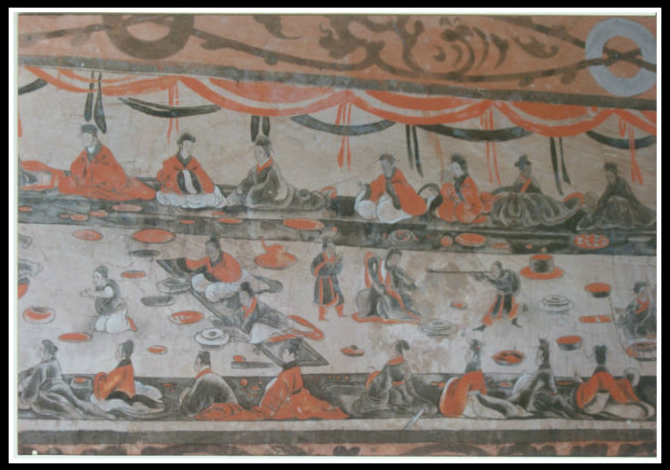
\includegraphics[width=0.6\linewidth]{Essen_in_Han_Dynastie}
\caption{汉朝时期的分桌而食}
\end{figure}

\begin{figure}
\centering
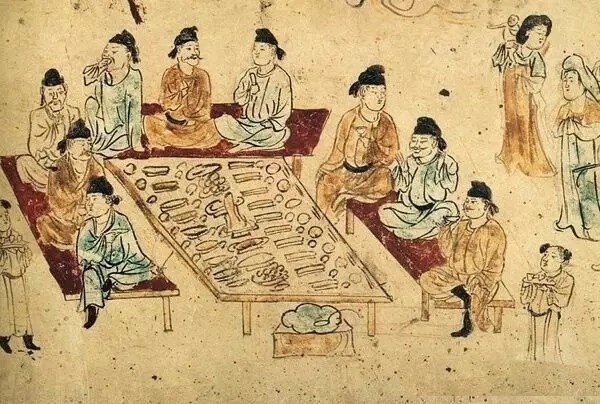
\includegraphics[width=0.45\linewidth]{Essen_in_Tang_Dynastie}
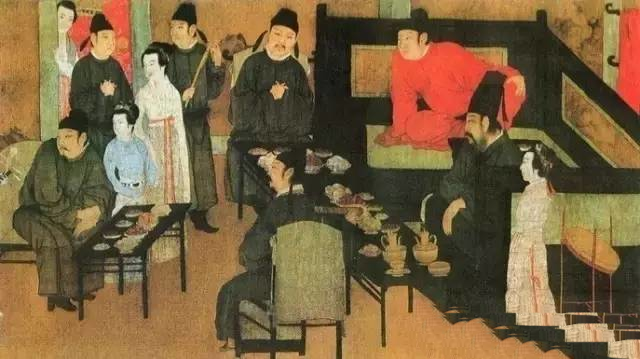
\includegraphics[width=0.45\linewidth]{Essen_in_song_Dynastie}
\caption{唐宋时期的合桌而食\protect\footnote{受北方少数民族影响唐宋时期人们平时宴饮开始围桌合餐。右图为北宋著名的韩熙夜宴图}}
\end{figure}
\par
分餐制在西方一直持续至今。文献记载从文艺复兴时期到维多利亚时代,欧洲贵族由佣人把菜端到桌子上,把大盘食物分到每个人的盘子里。而平民在厨房中吧食物分配好,再端到每个人面前。之所以分餐制能在贵族和平民之间如此流行。主要是因为⑴人们对注重饮食卫生的注重 ⑵曾经肆虐欧洲的黑死病,夺取了无数人们的生命,这种对黑死病的恐惧,深深植根在人们心中。⑶随着第一次与第二次工业革命的到来,极大的促进了社会的生产力,使人们更加富裕,使得在有钱人和贵族的分餐礼仪在中产阶级中流行起来。这样的分餐制也反应了欧洲文化的一种特点:人与人之间互不干扰,各负其责。
\begin{figure}
\centering
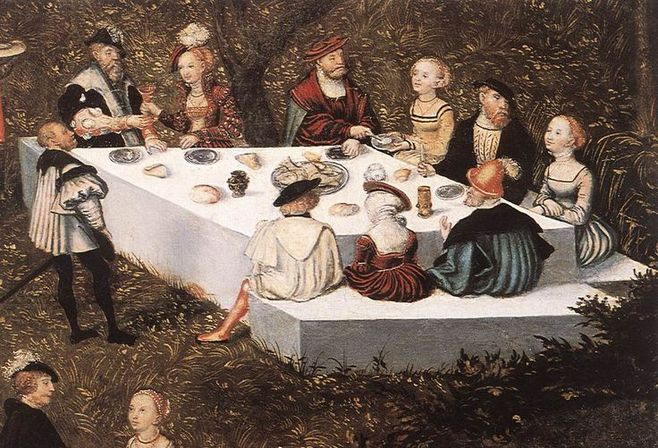
\includegraphics[width=0.45\linewidth]{Essen_in_Deutschland}
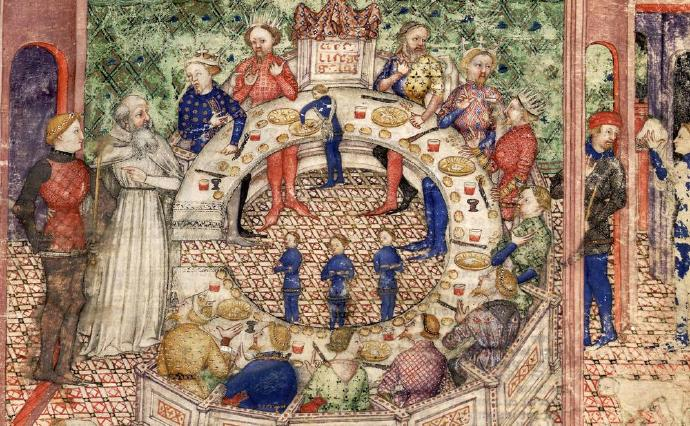
\includegraphics[width=0.45\linewidth]{Essen_in_Deutschland1}
\caption{欧洲人分餐的情形}
\end{figure}

\par
分餐与合餐是中德之间巨大的文化差异。德国:注重个人主义文化,独立自主,尊重隐私,理性分析和他人的利弊得失。而中方:注重集体主义,尊重互敬,爱护和支持关心他人。中国人喜欢给客人加菜,中国人认为这是人和人尊敬谦让的体现。而若是在德国,恐怕会被认为是个人的自由自主被侵犯。同时中国人在一张大桌上吃同一盘菜,难免会越身取食,在经过别人面前时,中国人不认为是不尊重的表现,反而是亲密关系的体现。这是文化中和谐包容的表现。而对于德国人会觉得私人空间被侵犯。因为德国的文化比较注重个人的隐私。
\par
从中德的餐桌文化差异,可以看到两国人民的文化特点。无论是中国还是德国,文化上都没有所谓的优劣,这些文化是中德两个国家的人民的智慧的结晶。他们像夜空中的繁星,点缀着人类文明的浩瀚银河。

\section{“你吃了吗?”}
基本在所有国家,一般两人见面,两人见面,都要问 :“你也好呢吧。回答:“好呢。”两人的对话就像写新闻消息的导语,接下来才谈正事。在德国也是如此,而在中国往往见面,特别是熟人见面时,所说的第一句话却是“你吃了吗?”。对中国来说这是一句非常真诚的问候,而不是限于礼节的客套。

在中国人看来,如果见面问候给人造成了心理压力,那对方回不回答彼此都很尴尬,所以,才有了约定俗成的这句“你吃了吗?”以其经典的特色延续了下来。大众广庭众目睽睽之下这样热情地一问,既体现了自己待人的热情,又不至于让对方难堪,也拉近了和对方的关系。

这一句问候的体现了中国饮食对中国人的重要性。所谓民以食为天,对于中国人来说吃是一等一的大事,尤其是在物资短缺的年代。饮食文化在与中国人民的交际中占有举足重轻的地位,主人宴请往往会给客人敬酒,夹菜,以示地主之谊。在中国,饮食已上升到了一种几乎超越其他一切物质形态和精神形态的举足轻重的东西。

中国传统的烹调方法,会因各大菜系的有所不同;同一菜点的口味不同风味与特点而主辅料的搭配,也会因为厨师的专长和喜好而有所不同,甚至还会因为厨师临场情绪的变化,做出某种即兴的发挥。这也体现中国文化,顺应自然,重视经验,轻视创新实验。

而在德国, 饮食仅仅作为一种生存的必要手段和交际方式。 林语堂先生曾说。 西方人的饮食观念不同于中国,英美人仅以“吃” 为对一个生物的机器注入燃料,保证其正常的运行,只要 他们吃了以后能保持身体健康、 结实,足以抵御病菌、 疾病的攻击,其他皆在不足道中。 不难看出,吃虽然重要,但是从文化的意义上看,在西方国家只是停留在简单的交流、 交际的层面上,并没有像在中国那样被赋予更多、更为重要的使命。

\subsection{ 主题拓展}
不仅仅是问候语,中国人的日常用语也有和饮食相关的表达:
\begin{enumerate}
\item 
职业 - 饭碗
\item
 幸福 - 陶醉
\item
 嫉妒 - 吃醋
\end{enumerate}
	\chapter{节日文化差异}
\section{节日禁忌} 

    “禁忌”一词来源于,国际学术界统称为“塔布”,源于太平洋小岛波利尼西亚汤加岛人的土语,音译为“taboo”或“Tabu”,其基本含义是表示“神圣的”、“不洁的”、和“危险的”、“不可接触的”。
    中国文化博大精深,然而在中国的传统文化当中有很多的禁忌,如果按照老一辈的人来说,这是老天爷安排的。按照现代人说,这就是迷信。但是无论是迷信是否,作文中国文化,我们更应该用继承的心态去面对。下面就介绍一些中国人在日常生活中碰到的或是不愿意去犯的禁忌。



\subsection{送礼禁忌}

    相信不止大家都为了挑选礼物而烦恼过,面对各种各样的节日,我们总是需要不停的购买适当的礼物送给对应的人,这个真的很让人苦恼。但是亲朋好友之间互相送礼物,更多的是为了传达一种祝福、表达一种诚意。用最近火热的词来说,就是一种“仪式感”。你挑选的礼物不一定真的符合你送礼对象的心意,或者也不是他们真正需要的。给同样的钱让他们自己买他们或许也不会买这个礼物,甚至你礼物送出去之后他们一辈子都不一定会用上一次。然而你在挑选礼物的过程中,已经投入了大量的精力和时间,而正是这些东西,会让对方感受到你的心意,这就是所谓的“礼轻情意重。”所以但是根据中国的风俗传统,送以下系类的礼物却可能会导致好心做坏事,也是众多礼物中比较忌讳的礼物:

    \begin{enumerate}
   \item 
   送结婚礼物时忌讳送“伞”、“钟”等物,因为“伞”与“散”谐音,散意离散,为人们所不喜欢,所以伞被视为不吉利的礼物,“钟”与“终”谐音,特别是“送钟”更会让老人们联想到“送终”,很不吉利。
   \item
   给病人送食品时也有谐音的禁忌。旧时上海去看望病人时,忌送苹果,因为上海话中“苹果”的发音与“病故”谐音。
   \item
   菊花常用于纪念逝者,不可以作为礼物送出。
   \item
   帽子俗话中有“愁帽子”之说,老人去世孝子要头戴孝帽,所以忌讳将帽子送给别人。特别是绿色的帽子,更是送礼的大忌。
   \item
   刀剑等利器,容易伤人,且俗话有“一刀两断”之说,用于送人恐有割断关系双方的不好联想,所以一般不作为礼品送人。
   \item
   扇子因为只用于夏天,一到秋凉天即被抛之不用,有绝情之意,俗称“送扇无相见”,所以不受欢迎,而且很多人会将“风扇”当成“分散”理解,潜台词就是分手。
   \item
   “鞋”与“邪”同音,而且鞋被踩在脚下,所以除了自己家人,一般不要给别人送鞋。
   \item
   ”梨“因为“梨”与“离”谐音,给夫妻、恋人不能送就很不适合。
   \item
   “镜子”与“禁子”谐音,且镜子易破易碎,所以也属于属送礼的忌讳之物。
        
    \end{enumerate}



\subsection{数字禁忌}

    数字不仅仅可以代表数量,还关联着不同语言文化、宗教信仰等深刻内涵。不同的国家地区都有着不同的数字禁忌,也有着不一样的数字偏好。如中国人就忌讳4,偏爱6、8、9。
    \begin{enumerate}
    \item 
    “四”谐音“死”,大凶,所以门牌号、车牌号都不宜有这个数字。过年的时候也忌说“4”、“死”等音的词。在日常生活中也能看到这样的例子:有很多外国人在中国生活久了之后都清楚在中国绝大部分大厦中是没有“4楼”的存在,通常是用“3A楼”或者“5A楼”来代替,或者直接就没有这一层楼,直接跳到了5楼。。这也是因为在中国的文字发音中间“4”和“死”同音,中国人普遍都忌讳死亡楼层。
    \item 
    数字当中,最吉利的要数六和八,所谓“六六大顺”、“要得发,不离八”,就说出了其中的原委。  
        
    \end{enumerate}



\subsection{谐音产生的禁忌}

    每年春节,全世界有超过十亿人加入庆祝的行列,并展开一场微妙的文字游戏。它很像一组求爱仪式——为了招来好运,人们会用喜庆字样的剪纸来装点住宅与门户。要理“发”的,年前赶紧理完,谁想在新年伊始削去财运,哪怕只是稍事修剪?年夜饭的菜肴里通常有鱼,因为人们希望“年年有余”;有的地方还时兴吃一种名为发菜的藻类,因为谐音“发财”;或有“橙”,寓意为“成”,所以在春节的装饰物中常常可以看见柑橘类水果的身影。而且有研究表明,在中文语境下,人们对同音歧义似乎更为敏感。

   (1)如在亲友结婚之日,忌讳说“死、光、输、完、离、散、休”等不吉利字词。

   (2)在结婚时,新娘上门禁吃瓜类,因为“瓜”与“寡”谐音,以免将来做寡妇。

   (3)和亲友一起吃梨时不能分吃一个梨,因为“分梨”与“分离”谐音。

   (4)沿海渔民或船家忌说“沉”、“箸”等字。因为“沉”和“沉船”的沉同音同字,因此人们把“沉”字改说“重”字。吃饭用的“箸”与“住”谐音,即停住抛锚之意,对行船来说是不吉利的。因此人们把吃饭时用的“箸”改称“筷子”,取“筷”与“快”的谐音,即“快”行、“一帆风顺”之意。

   (5)在广州一带,人们把“猪舌”称作“猪月利”,由于广东话中“舌”与“蚀”同音,经商者忌讳蚀本,改称“猪月利”则含“月月盈利”的意思。北京话“舌”与“折”同音,也有“折本”不吉利之嫌,因此北京、天津等地把“猪舌”称作“口条”。广州人把丝瓜称作“胜瓜”,因为广州话“丝”与“输”谐音。广东潮汕一带把“药”称作“利市”或“甘茶”,而忌说“药”字,因为“药”与“病”相关,所以把有病“服药”叫“辗利市”或“服甘茶”。



\subsection{其他}

    除了上文中的禁忌之外,中国人在日常生活中还有许多有趣的禁忌。
    
   (1)在中国写别人名字的时候十分忌讳用红笔书写。
   这一点在老一辈人中间特别在意,在他们看来红色墨水写出来的字颜色接近血色,是带有诅咒的意思,如果用红色墨水写一个人的名字将会给这个人带了厄运,所以很多的老师在小学的时候就会告诉小孩子不要用红笔写名字。

   (2)吃饭的时候所有人都忌讳将筷子竖拆在饭碗中间。
   第二个几乎是所有中国小孩都喜欢做的事情,但是无一例外都被家长斥责过。在中国是习惯吃米饭的,不像西方国家吃饭是都是使用刀叉,在中国使用的餐具基本上都是筷子,在吃饭的时候所有人都忌讳将筷子竖拆在饭碗中间,这种现象在别人看来几乎是和祭拜死人没什么差别,所有人都十分忌讳,除此之外也不能在吃饭的时候用筷子指着别人。

   (3)忌讳在家里种柳树。
   柳树,想必大家都很熟悉了,一种非常漂亮的树,一条条柳条随风飘摇。但是这种树虽然很好看,但是有没有小伙伴们注意到,这么漂亮的树一般很少出现在私人庭院或是哪个企业的庭院之中。因为从古至今,在民间人们都说,柳树是极阴之物,一般很少人会去接近柳树,即便是很好看也只是站在较远的地方观赏。正因为柳树是极阴之物,所以在夜晚甚至是白天的时候,会引得很多孤魂野鬼在柳树底下吸食阴气。如果有人在柳树底下呆久了,运气不好的话很有可能被冤鬼缠上,而且在阴气较重的地方呆久了,阴气入体,轻则大病一场,重则一命呜呼。也正是柳树是嫉阴之物,所以在古代民间很多道士或是先生那里都会准备一些柳条,因为柳条是可以直接抽鬼的,就像用鞭子抽人一样,有着驱鬼的功能。

   (4)通灵的狗。
   大家都知道,狗是我们人类的最好的伙伴,从各方面来讲,狗是非常容易驯服并且利用的动物。相信很多人也知道,狗的眼睛是通灵的,能看到一些人所看不到的一些东西,经常走在路上或是在晚上半夜的时候突然一下就狂吠不止,那这就说明附近肯定就有不干净的东西了。在古代的一些民间说法是如果半夜1-3点,阴气正中的时候,突然狗跳起来狂吠十几下,那多半就是有什么孤魂野鬼从旁边经过了。如果这只狗一直狂吠不停,时间长达半个多小时,那么多半就是遇见了什么孤魂野鬼停留在了附近久久不愿离去。如果狗在狂吠的时候,时不时的站立了起来,然后尾巴夹的仅仅的,那么狗所看到的灵体多半是厉鬼或是冤魂。如果狗表现的全身发抖,吼两声就低声“哼哼”,然后时不时的往后退,眼睛里充满着泪水,那证明狗看到了不一般的灵体,估计是什么怨念极深的厉鬼,类似于罗刹鬼母这种级别的冤鬼,这时候的你要做的就是立马撒丫子狂奔,以免被缠上。如果被缠上了,没得谈,阎王老子也救不了你。

   (5)外地旅游入住酒店过夜时一定要彻夜开灯。
   老一辈们认为酒店是个怨气很重的场所,每当半夜时分都会出现一些灵异现象,比如听到婴儿哭声、鬼压床等。但这些“赃东西”都是怕光的,所以在酒店过夜时一定要彻夜开灯。当然了,若自己不喜欢在卧室开灯睡觉的话,也可以把厕所的灯开。

   (6)晚上外出时不要去踩别人的影子。
   我们吃完晚饭后都会有出去散步的习惯,在这提醒一下大家,一定不要去踩别人的影子或者自己的影子被别人踩!相传影子是灵魂的表现形式之一,若踩到了会对灵魂造成“创伤”!若自己失去了影子,那么就意味着自己变成了鬼,因为鬼是没有影子的!

   (7)床不能对着镜子。
   镜子在夜晚的时候,还会反射出人们的倒影,这样一来,就会影响到我们的行为,因为夜晚上厕所的话,就会看到镜中憔悴的自己,这样一来,夫妻之间就会出现裂痕,那么吵架也是在所难免的事情了。其实床对着镜子本身就是一种不好的结构,所以一定要对镜子的摆放位置非常敏感,才能够帮助到我们在日常生活中,生活得更加美好。

   (8)不能敲饭碗。
   敲碗首先会显得没有教养。比如去别人家作客,假如敲碗,那么意思就是在催主人快点,等不及了。其次是民间有种说法,说吃饭敲碗,以后生活会不好,会出去乞讨,因为乞丐要饭才敲碗。



   “十里不同风,百里不同俗”,在中国,各民族、各地区都有千姿百态的民俗。民俗是民间记忆的载体,反映了普通民众在历史长河中不断发展、变化的生产、生活情境以及蕴含在其中的精神与情感,是中国传统文化的重要组成部分。中国有五千年的历史,从迷信走到了科学,但是每个地方还是有老辈人口传下来的忌讳,如人的一生以36岁为大忌,每个人到了35就不做比较危险的工作,就是做什么事都比较小心点,一直到37就可以了,很多人连36这个数字都很忌讳,买卖东西不可以出现36,少给都可以,不然准挨骂,还有很多,譬如打牌的人不可以买红色的包包,过年吃团圆饭的时候严禁别人串门,又譬如一串很忌讳的老话,正月不见鹰打鸟,二月不见狗擦裆,三月不见蛇吸雾,四月不见人成双,就是看见了就会有灾难找上门。这些中国各地在不同期间的不同的习俗和禁忌,也是非常有趣又有意义的,这也是我们民族文化传统的一部份,值得世代流传。

	
\end{document}